\documentclass[10pt,english,a4paper]{article}
\usepackage[utf8]{inputenc}
\usepackage[T1]{fontenc}
\usepackage{babel}

\usepackage[svgnames]{xcolor}
\usepackage{a4wide}
\usepackage{graphicx}
\usepackage{url}
\usepackage{eurosym}
\usepackage{vmargin}
\usepackage{fancyhdr}
\usepackage{multicol}
\usepackage{lastpage}
\usepackage{eso-pic}
\usepackage{listings}
\usepackage{hyperref}
\usepackage{longtable}
\usepackage{syntax}
\usepackage{xspace}

\setlength{\grammarindent}{11em}

\synctex=1

\newcommand\tup[1]           {\langle#1\rangle}
\newcommand\set[1]           {{\{ #1 \mathclose \}}}
\newcommand\ctla             {\textbf{A}\xspace}
\newcommand\ctle             {\textbf{E}\xspace}
\newcommand\ltlf             {\textbf{F}\xspace}
\newcommand\ltlg             {\textbf{G}\xspace}
\newcommand\ltlx             {\textbf{X}\xspace}
\newcommand\ltlu             {\textbf{U}\xspace}
\newcommand\logicnot         {\boldmath$\lnot$\xspace}
\newcommand\logicand         {\boldmath$\land$\xspace}
\newcommand\logicor          {\boldmath$\lor$\xspace}
\newcommand\atomleq          {\boldmath$\leq$\xspace}
\newcommand\atomdead         {\textbf{deadlock}\xspace}
\newcommand\atomisfire[1]    {\textbf{is-fireable}(#1)}
\newcommand\atomplacebnd[1]  {\textbf{place-bound}(#1)}
\newcommand\atomtokenscnt[1] {\textbf{token-count}(#1)}
\newcommand\exprplus         {\boldmath$+$\xspace}
\newcommand\exprminus        {\boldmath$-$\xspace}


\newcommand{\CC}{%
  C\nolinebreak\hspace{-.05em}\raisebox{.4ex}{\scriptsize\bf +}\nolinebreak\hspace{-.10em}\raisebox{.4ex}{\scriptsize\bf +}%
}

%\definecolor{listinggray}{gray}{0.92}
\lstdefinelanguage{rnc}
{ morekeywords={element, complexType, sequence, ID, IDREF, complexContent, extension, attribute}
, morekeywords=[2]{name, minOccurs, maxOccurs, ref, type, substitutionGroup, base, abstract}
, morekeywords=[3]{xs, mcc}
, basicstyle=\scriptsize\fontfamily{fvm}\selectfont
, keywordstyle=\scriptsize\fontfamily{fvm}\selectfont\color{Purple}
, keywordstyle=[2]\scriptsize\fontfamily{fvm}\selectfont\color{DarkBlue}
, keywordstyle=[3]\scriptsize\fontfamily{fvm}\selectfont\color{ForestGreen}
, stringstyle=\scriptsize\fontfamily{fvm}\selectfont\color{FireBrick}
, morestring=[b]"
, backgroundcolor=\color{blue!10}
}
\lstset{
  rulecolor=\color{black}
, breaklines=true
, tabsize=2
, flexiblecolumns=false
, keywordstyle=\bfseries
, basicstyle=\scriptsize\ttfamily
, xleftmargin=1cm
, xrightmargin=1cm
, language=rnc
}
\lstdefinelanguage{xsd}
{ morekeywords={element, complexType, sequence, ID, IDREF, complexContent, extension, attribute}
, morekeywords=[2]{name, minOccurs, maxOccurs, ref, type, substitutionGroup, base, abstract}
, morekeywords=[3]{xs, mcc}
, basicstyle=\scriptsize\fontfamily{fvm}\selectfont
, keywordstyle=\scriptsize\fontfamily{fvm}\selectfont\color{Purple}
, keywordstyle=[2]\scriptsize\fontfamily{fvm}\selectfont\color{DarkBlue}
, keywordstyle=[3]\scriptsize\fontfamily{fvm}\selectfont\color{ForestGreen}
, stringstyle=\scriptsize\fontfamily{fvm}\selectfont\color{FireBrick}
, morestring=[b]"
, backgroundcolor=\color{blue!10}
}
\lstdefinelanguage{mpl}
{ basicstyle=\scriptsize\fontfamily{fvm}\selectfont
, keywordstyle=\scriptsize\fontfamily{fvm}\selectfont\color{Purple}
, stringstyle=\scriptsize\fontfamily{fvm}\selectfont\color{FireBrick}
, morestring=[b]"
, backgroundcolor=\color{green!10}
}

\definecolor{rulercolor}{RGB}{255,255,255}
\definecolor{sectioncolor}{RGB}{50,50,50}
\definecolor{defaultcolor}{RGB}{100,37,16}

\oddsidemargin = 1cm
\evensidemargin = 1cm
\textwidth = 19cm
\topmargin = 1.2cm
\textheight = 24cm
\parskip = 0.1cm
\parindent = 0.0cm

%%%%%%%%%%%%%%%%%%%%%%%%%%%%%%%%%%%%%%%%%%%%%%%%%%%%%%
\fancyhf{}

\renewcommand{\headrulewidth}{0pt}
\renewcommand{\footrulewidth}{0pt}

\lhead{\textcolor{rulercolor}{Model Checking Contest @ Petri Nets}\\\ \\}
\chead{\textcolor{rulercolor}{Page {\thepage}/\pageref{LastPage}}\\\ \\}
\rhead{\textcolor{rulercolor}{Property Language Manual}\\\ \\}

\lfoot{}
\cfoot{}
\rfoot{}
%%%%%%%%%%%%% pour un fond
\newcommand\BackgroundPic{
\put(0,-160){
\parbox[b][\paperheight]{\paperwidth}{%
\vfill
\centering
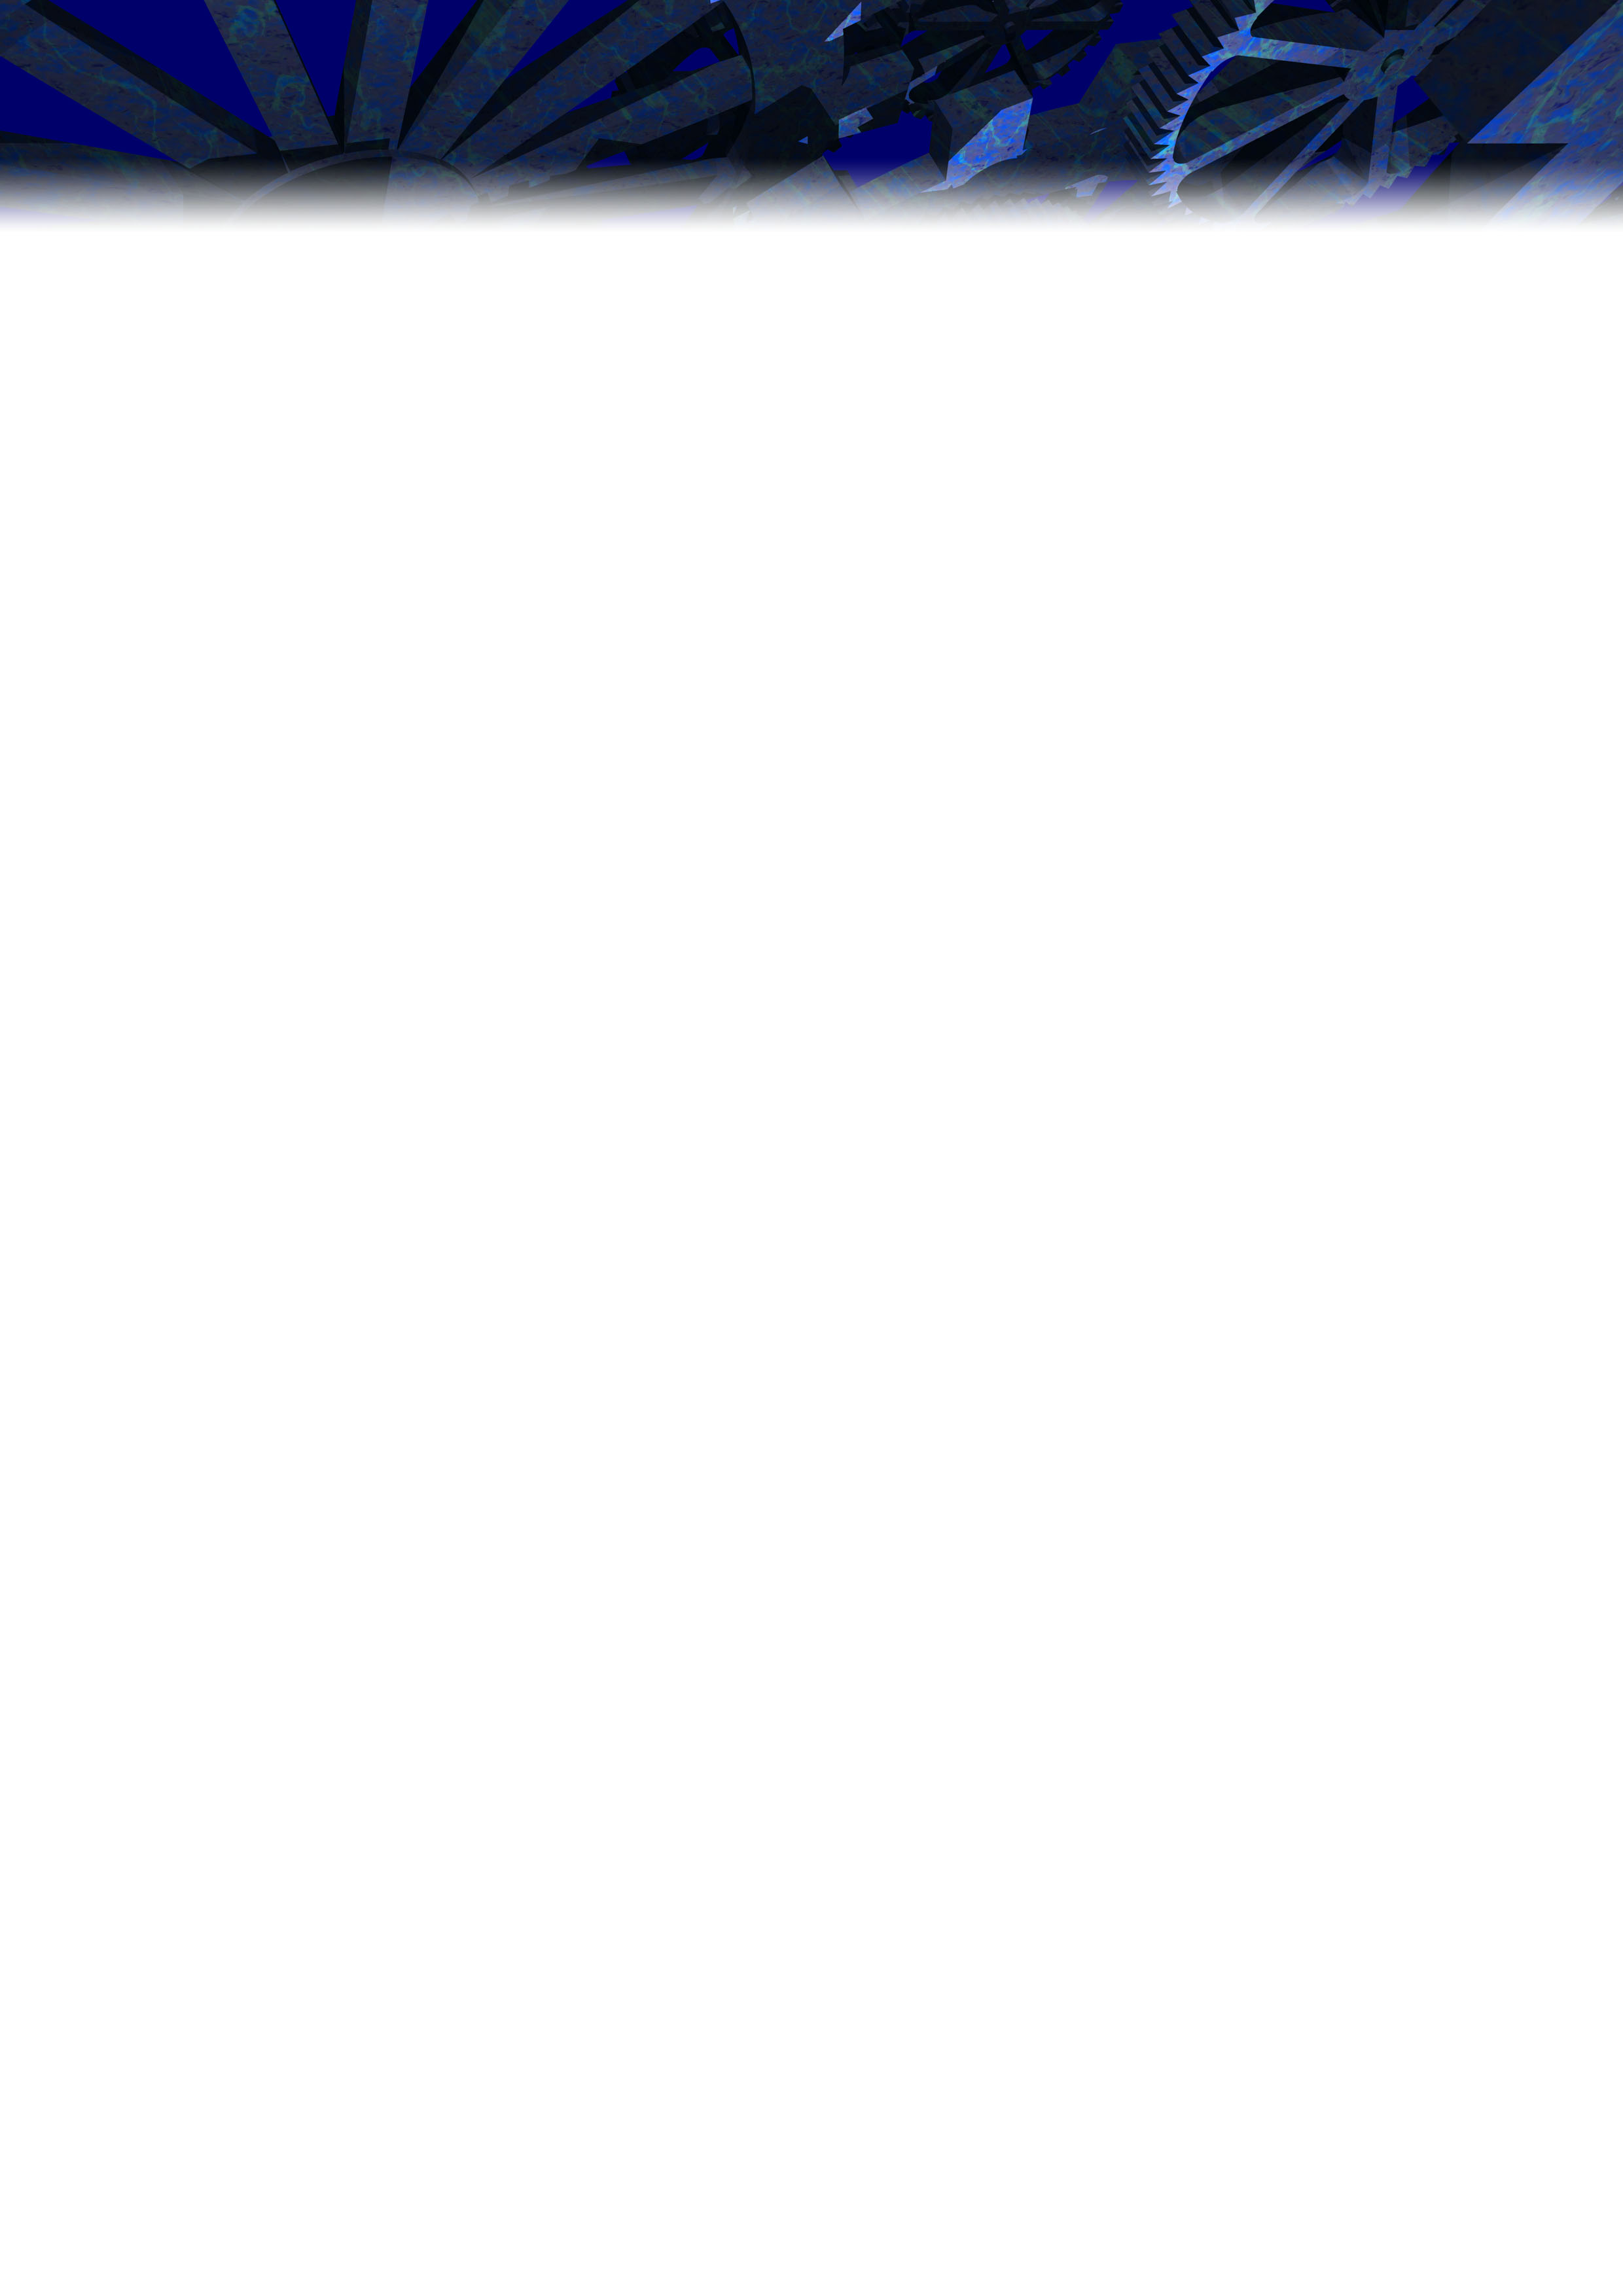
\includegraphics[width=23.5cm,keepaspectratio]{background2015.jpg}%
\vfill
}}}
%%%%%%%%%%%%%%%%%%%%%%%%% fin fond

\renewcommand{\rmdefault}{phv}
\renewcommand{\sfdefault}{cmr}
%\renewcommand{\ttdefault}{pcr}

%%%%%%%%%%%%%%%%%%%%%%%%%%%%%%%%%%%%
\newcommand{\fk}[1]{\color{blue}FK: #1\color{defaultcolor}\ }
\newcommand{\fp}[1]{\color{red}FK: #1\color{defaultcolor}\ }

\newcommand{\mcc}[0]{MCC}
\newcommand{\mccl}[0]{Model Checking Contest @ Petri Nets}
%%%%%%%%%%%%%%%%%%%%%%%%%%%%%%%%%%%%

\newcommand\myparagraph[1]{\color{sectioncolor}\smallskip\textbf{#1. }\color{defaultcolor}}
\newcommand\mysection[1]{\color{sectioncolor}\section{#1}\color{defaultcolor}}
\newcommand\mysubsection[1]{\color{sectioncolor}\subsection{#1}\color{defaultcolor}}

\pagestyle{fancy}
\AddToShipoutPicture{\BackgroundPic}

\begin{document}
\color{defaultcolor}

\section*{Goals of the property language}
The property language for the \mcc{} @ Petri Nets is a language designed to allow
participation of many tools.
It allows to write structural, reachability, CTL, LTL formul{\ae}.
It is tightly related to Petri nets, that are the modeling formalism used during the contest.

This language is designed to evolve in the future editions of the contest.
It is also designed to integrate with Petri Net Markup Language in the future.
To do so, the language is provided as a RelaxNG grammar and an XML Schema generated from it.

This document presents this language in two steps: first an informal presentation of the grammar of the language of formulæ used to define properties (and the sublanguages of all the particular categories in which tools can compete at the MCC), and then a description of how these properties are defined in practice and how they can be interfaced with a tool.

Notice that, with simplification in mind, this year property language is a subset of last year language. Any tool which was participating in last year MCC should thus be able to deal with this language. 

\tableofcontents
\clearpage

\section{Informal grammars for the formulæ}

Each property used in the MCC is defined by a formula on the places and the transitions of the corresponding Petri net. These formulæ follow the general grammar informally presented below, where A (along all paths) and E (there exists a path) are the standard CTL operators, G (globally), F (finally), X (next), and U (until) are the standard LTL operators, $\lnot$ (not), $\wedge$ (and), and $\vee$ (or) are standard boolean operators, $\leq$ (less or equal), $+$ (plus), and $-$ (minus) are standard integer arithmetic operators.
The predicate \emph{deadlock} stands for ``the current state is a deadlock'' and the predicate \emph{is-fireable($t_1$,\dots,$t_n$)} stands for ``one of the set of transitions $\{t_1,\dots,t_n\}$ is fireable from the current state''.
Finally, \emph{integer-constant} is any integer, \emph{tokens-count($p_1$,\dots,$p_n$)} gives the total number of tokens in the places $p_1$ to $p_n$ at the current state, and \emph{place-bound($p_1$,\dots,$p_n$)} gives the maximum of \emph{tokens-count($p_1$,\dots,$p_n$)} over all (reachable) states.

\begin{grammar}
<formula> ::= <boolean-formula>
\alt <integer-formula>

<boolean-formula> ::= \ctla <boolean-formula>
\alt \ctle <boolean-formula>
\alt \ltlg <boolean-formula>
\alt \ltlf <boolean-formula>
\alt \ltlx <boolean-formula>
\alt <boolean-formula> \ltlu <boolean-formula>
\alt \logicnot <boolean-formula>
\alt <boolean-formula> \logicand <boolean-formula>
\alt <boolean-formula> \logicor <boolean-formula>
\alt <atom>

<atom> ::= \atomdead
\alt \atomisfire{$t_1, \ldots, t_n$}
\alt <integer-expression> \atomleq <integer-expression>

<integer-formula> ::= <integer-expression>

<integer-expression> ::=
     <integer-expression> \exprplus <integer-expression>
\alt <integer-expression> \exprminus <integer-expression>
\alt \textit{Integer constant}
\alt \atomplacebnd{$p_1, \ldots, p_n$}
\alt \atomtokenscnt{$p_1, \ldots, p_n$}

\end{grammar}

FIXME all integer constants are 0, 1, 2

This grammar defines a large class of formulæ.
For the MCC, these formulæ are grouped among several subclasses, each one corresponding to a restriction of the above grammar.
Each of these subclasses defines a particular category and the tools are tested in each of these category independently.
For each category of formulæ used at MCC we specify below the restriction of the above grammar that will be used.
Each category is designated by the name of the XML file providing the formulæ from this category (how formulæ are defined as XML files is the topic of the next Sections of this manual).

%
%
% parler du lien entre fichiers xml et tool submission kit (i.e. pour chaque modele il y aura chaque fichier de formules)
%
%
%

\subsection{Category \textit{ReachabilityDeadlock}}

\begin{grammar}

<formula> ::= <boolean-formula>

<boolean-formula> ::= \ctle \ltlf \atomdead
%\alt A G $\lnot$ deadlock

\end{grammar}

\subsection{Category \textit{ReachabilityFireabilitySimple}}

\begin{grammar}

<formula> ::= <boolean-formula> 

<boolean-formula> ::= \ctle \ltlf \atomisfire{$t_1, \ldots, t_n$}
\alt \ctla \ltlg \atomisfire{$t_1, \ldots, t_n$}

\end{grammar}

\subsection{Categories \textit{ReachabilityFireability} and \textit{ReachabilityCardinality}}

Both categories contain formulas produced using the same grammar, the only
difference being the atomic propositions allowed in each one.
The grammar is the following:

\begin{grammar}
<formula> ::= <boolean-formula>

<boolean-formula> ::= \ctle \ltlf <state-formula>
\alt \ctla \ltlg <state-formula>

<state-formula> ::=  \logicnot  <state-formula>
\alt <state-formula> \logicand <state-formula>
\alt <state-formula> \logicor  <state-formula>
\alt <atom>
\end{grammar}

Now, the cateory \emph{ReachabilityFireability} only contains
\atomisfire{$\cdot$} atoms:

\begin{grammar}
<atom> ::= \atomisfire{$t_1, \ldots, t_n$}
\end{grammar}

while the formulas in the \emph{ReachabilityCardinality} category contain
integer inequalities:

\begin{grammar}
<atom> ::= <integer-expression> \atomleq <integer-expression>

<integer-expression> ::= \textit{Integer constant}
\alt \atomtokenscnt{$p_1, \ldots, p_n$}
\end{grammar}

Recall that the \textit{Integer constant} will be a number in $\set{0,1,2}$.

\subsection{Category \textit{ReachabilityBounds}}

\begin{grammar}

<formula> ::= <boolean-formula>

<boolean-formula> ::=  \logicnot <boolean-formula>
\alt <boolean-formula> \logicand <boolean-formula>
\alt <boolean-formula> \logicor  <boolean-formula>
\alt <atom>

<atom> ::= <integer-expression> \atomleq <integer-expression>

<integer-expression> ::= \textit{Integer constant}
\alt \atomplacebnd{$p_1, \ldots, p_n$}

\end{grammar}

\subsection{Cateogory \textit{ReachabilityComputeBounds}}

Observe that this is the only category where formulas evaluate to an
integer number rather than a boolean value.

\begin{grammar}
<formula> ::= <integer-formula>

<integer-formula> ::= \atomplacebnd{$p_1, \ldots, p_n$}
\end{grammar}


\subsection{Category \textit{LTLFireabilitySimple}}

\begin{grammar}
<formula> ::= <boolean-formula>

<boolean-formula> ::= \ctla <path-formula>

<path-formula> ::=
     \ltlg <atom>
\alt \ltlf <atom>
\alt \ltlx <atom>
\alt <atom> \ltlu <atom>

<atom> ::= \atomisfire{$t_1, \ldots, t_n$}
\end{grammar}

\subsection{Categories \textit{LTLFireability} and \textit{LTLCardinality}}

Both categories contain formulas produced using the same grammar, the only
difference being the atomic propositions allowed in each one.
The grammar is the following:

\begin{grammar}

<formula> ::= <boolean-formula>

<boolean-formula> ::= \ctla <path-formula>

<path-formula> ::=
     \ltlg <path-formula>
\alt \ltlf <path-formula>
\alt \ltlx <path-formula>
\alt <path-formula> \ltlu <path-formula>
\alt <atom>

\end{grammar}

Now, the category \emph{LTLFireability} only contains \atomisfire{$\cdot$} atoms:

\begin{grammar}
<atom> ::= \atomisfire{$t_1, \ldots, t_n$}
\end{grammar}

while the formulas in the \emph{LTLCardinality} category contain integer
inequalities:

\begin{grammar}
<atom> ::= <integer-expression> \atomleq <integer-expression>

<integer-expression> ::= \textit{Integer constant}
\alt \atomtokenscnt{$p_1, \ldots, p_n$}
\end{grammar}


\subsection{Category \textit{CTLFireabilitySimple}}

\begin{grammar}
<formula> ::= <boolean-formula>

<boolean-formula> ::= \ctla <path-formula>
\alt \ctle <path-formula>

<path-formula> ::=
     \ltlg <atom>
\alt \ltlf <atom>
\alt \ltlx <atom>
\alt <atom> \ltlu <atom>

<atom> ::= \atomisfire{$t_1, \ldots, t_n$}
\end{grammar}

\subsection{Cateogries \emph{CTLFireability} and \emph{CTLCardinality}}

Both categories contain formulas produced using the same grammar, the only
difference being the atomic propositions allowed in each one.
The grammar is the following:

\begin{grammar}
<formula> ::= <boolean-formula>

<boolean-formula> ::=
     \ctla <path-formula>
\alt \ctle <path-formula>
\alt \logicnot <boolean-formula>
\alt <boolean-formula> \logicand <boolean-formula>
\alt <boolean-formula> \logicor <boolean-formula>
\alt <atom>

<path-formula> ::=
     \ltlg <boolean-formula>
\alt \ltlf <boolean-formula>
\alt \ltlx <boolean-formula>
\alt <boolean-formula> \ltlu <boolean-formula>
\end{grammar}

The cateory \emph{CTLFireability} only contains \atomisfire{$\cdot$} atoms:

\begin{grammar}
<atom> ::= \atomisfire{$t_1, \ldots, t_n$}
\end{grammar}

while the formulas in the \emph{CTLCardinality} category contain
integer inequalities:

\begin{grammar}
<atom> ::= <integer-expression> \atomleq <integer-expression>

<integer-expression> ::= \textit{Integer constant}
\alt \atomtokenscnt{$p_1, \ldots, p_n$}
\end{grammar}

Observe that under the previous definitions it is possible to derivate a
formula without any CTL operator, by using the last grammar production for
the non-terminal \synt{boolean-formula}.
However, such formul{\ae} will never be presented to a tool participating
in these categories, we will ensure that
\emph{formul{\ae} contain at least one CTL (either \ctla or \ctle)
operator}.

\clearpage
\section{Description of the property language as a RelaxNG grammar}

The property language is designed as a RelaxNG grammar. Thus, properties are given in XML.
We generate a text equivalent from it, but it is not stable and only given for readability.
As an introducing example, consider the following property, given in XML (left) and the corresponding formula as it could be generated by the above informal grammar (right).

\begin{multicols}{2}
\begin{lstlisting}
   <?xml version="1.0"?>
   <property-set xmlns="http://mcc.lip6.fr/">
    <property>
     <id>Dekker-PT-010-test1</id>
     <description>
      Automatically generated formula.
     </description>
     <formula>
      <exists-path>
       <until>
        <before>
         <negation>
          <integer-le>
           <integer-constant>1</integer-constant>
           <tokens-count>
            <place>p3_0</place>
           </tokens-count>
          </integer-le>
         </negation>
        </before>
        <reach>
         <is-fireable>
          <transition>withdraw_4_8</transition>
         </is-fireable>
        </reach>
       </until>
      </exists-path>
     </formula>
    </property>
   </property-set>
\end{lstlisting}
\columnbreak
\footnotesize
\vspace*{2cm}
E (($\lnot$ (1 $\leq$ tokens-count(p3\_0))) U is-fireable(withdraw\_4\_8))
\end{multicols}

Below is the description of the RelaxNG grammar we use to generate such properties.


\begin{lstlisting}
  default namespace = "http://mcc.lip6.fr/"
  start = property-set
\end{lstlisting}
\subsection{Property sets}
The \lstinline[language=xsd]!property-set! element is the root of the XML representation.
It contains several properties.
\begin{lstlisting}
  default namespace = "http://mcc.lip6.fr/"
  start = property-set

  property-set = element property-set {
    property*
  }
\end{lstlisting}

\subsection{Properties}
A property is composed of three mandatory parts: a unique identifier, a textual description
of the property, and a formula.
%It has a set of tags to give a hint about the class of tools that can compute the formula
%(structural, reachability, CTL or LTL). These hints do \emph{not} say that the formula
%is expressed exactly in the language given by the hint, but tells that given minor changes,
%it could be.

%A property also contains an optional part for the expected result.
%It gives the expected value and a textual explanation.
%% \begin{lstlisting}
%%   property = element property {
%%     element id {
%%       xsd:ID
%%     } &
%%     element description {
%%       text
%%     } &
%%     element tags {
%%       element is-structural { xsd:boolean } &
%%       element is-reachability  { xsd:boolean } &
%%       element is-ctl { xsd:boolean } &
%%       element is-ltl { xsd:boolean }
%%     } &
%%     element expected-result {
%%       element value {
%%         xsd:integer | xsd:boolean
%%       } &
%%       element explanation {
%%         text
%%       }
%%     }? &
%%     element formula {
%%       formula
%%     }
%%   }
%% \end{lstlisting}

\begin{lstlisting}
  property = element property {
    element id {
      xsd:ID
    } &
    element description {
      text
    } &
    element formula {
      formula
    }
  }
\end{lstlisting}


\subsection{Formul{\ae}}
Formul{\ae} are the body of properties.
They define what is expected to hold on the model.
Formulas are currently of two main types: formul{\ae} that return integers, and formul{\ae}
that return Booleans.

In the following, for each rule of the grammar defining formulæ we give the RelaxNG representation (on the left) as well as the corresponding part of the informal grammar for formulæ of the previous Section (on the right).


\begin{multicols}{2}
\begin{lstlisting}
  formula =
      boolean-formula
    | integer-formula
\end{lstlisting}
\columnbreak
\scriptsize
\scriptsize\begin{grammar}
<formula> ::= <boolean-formula>
\alt <integer-formula>
\end{grammar}
\end{multicols}

%\clearpage
\subsection{Boolean formul{\ae}}

Boolean formul{\ae} are the majority of available formul{\ae}.
We define them in several parts.

\begin{lstlisting}
  boolean-formula = ...
\end{lstlisting}

%% \subsubsection{Reachability operators}

%% \begin{lstlisting}
%%   boolean-formula =
%%       ...
%%     | element invariant {
%%         boolean-formula
%%       }
%%     | element impossibility {
%%         boolean-formula
%%       }
%%     | element possibility {
%%         boolean-formula
%%       }
%%     | ...
%% \end{lstlisting}

%% \begin{itemize}
%%   \item \lstinline!invariant! evaluates to true if its subformula
%%     is verified for all states of the system;
%%   \item \lstinline!impossibility! evaluates to true if its subformula
%%     is never verified for all states of the system;
%%   \item \lstinline!possibility! evaluates to true if its subformula
%%     is verified for some states of the system (at least one).
%% \end{itemize}

\subsubsection{State operators}

These operators are the \lstinline!A! and \lstinline!E! operators of CTL.

\begin{multicols}{2}
\begin{lstlisting}
  boolean-formula =
      ...
    | element all-paths {
        boolean-formula
      }
    | element exists-path {
        boolean-formula
      }
    | ...
\end{lstlisting}
\columnbreak
\scriptsize
\scriptsize\begin{grammar}
<boolean-formula> ::= A <boolean-formula>
\alt E <boolean-formula>
\end{grammar}
\end{multicols}

\subsubsection{Path operators}

These operators are the \lstinline!X!, \lstinline!G!, \lstinline!F! and \lstinline!U!
operators of CTL and LTL.

%% \begin{lstlisting}
%%   boolean-formula =
%%       ...
%%     | element globally {
%%         boolean-formula
%%       }
%%     | element finally {
%%         boolean-formula
%%       }
%%     | element next {
%%         boolean-formula &
%%         element if-no-successor { xsd:boolean } &
%%         element steps { xsd:positiveInteger }
%%       }
%%     | element until {
%%         element before {
%%           boolean-formula
%%         } &
%%         element reach {
%%           boolean-formula
%%         } &
%%         element strength {
%%           "weak" | "strong"
%%         }
%%       }
%%     | ...
%% \end{lstlisting}

\begin{multicols}{2}
\begin{lstlisting}
  boolean-formula =
      ...
    | element globally {
        boolean-formula
      }
    | element finally {
        boolean-formula
      }
    | element next {
        boolean-formula &
    | element until {
        element before {
          boolean-formula
        } &
        element reach {
          boolean-formula
        } &
      }
    | ...
\end{lstlisting}
\columnbreak
\scriptsize
\scriptsize\begin{grammar}
<boolean-formula> ::= G <boolean-formula>
\alt F <boolean-formula>
\alt X <boolean-formula>
\alt <boolean-formula> U <boolean-formula>
\end{grammar}
\end{multicols}


\begin{itemize}
  \item \lstinline!next! should evaluate to false if no successor state exists;
  %\item \lstinline!until! has a \lstinline!strength! modifier, allowing the weak until.
\end{itemize}

\subsubsection{Petri net operators}

\begin{multicols}{2}
\begin{lstlisting}
  boolean-formula =
      ...
    | element deadlock { empty }
    | element is-fireable {
        transition+
      }
    | ...
\end{lstlisting}
\columnbreak
\scriptsize\begin{grammar}
<boolean-formula> ::= deadlock
\alt is-fireable($t_1$,\dots,$t_n$)
\end{grammar}
\end{multicols}


\begin{itemize}
  \item \lstinline!deadlock! evaluates to true if the current state is a deadlock
    (has no successor);
  \item \lstinline!is-fireable! evaluates to true if one of the set of transitions given
    is fireable from the current state.
\end{itemize}

\subsubsection{Boolean operators}

These are usual Boolean operators.

%% \begin{lstlisting}
%%   boolean-formula =
%%       ...
%%     | element true  { empty }
%%     | element false { empty }
%%     | element negation {
%%         boolean-formula
%%       }
%%     | element conjunction {
%%         boolean-formula,
%%         boolean-formula+
%%       }
%%     | element disjunction {
%%         boolean-formula,
%%         boolean-formula+
%%       }
%%     | element exclusive-disjunction {
%%         boolean-formula,
%%         boolean-formula+
%%       }
%%     | element implication {
%%         boolean-formula,
%%         boolean-formula
%%       }
%%     | element equivalence {
%%         boolean-formula,
%%         boolean-formula+
%%       }
%%     | ...
%% \end{lstlisting}

\begin{multicols}{2}
\begin{lstlisting}
  boolean-formula =
      ...
    | element negation {
        boolean-formula
      }
    | element conjunction {
        boolean-formula,
        boolean-formula+
      }
    | element disjunction {
        boolean-formula,
        boolean-formula+
      }
    | ...
\end{lstlisting}
\columnbreak
\scriptsize\begin{grammar}
<boolean-formula> ::= $\lnot$ <boolean-formula>
\alt <boolean-formula> $\wedge$ <boolean-formula>
\alt <boolean-formula> $\vee$ <boolean-formula>
\end{grammar}
\end{multicols}


\subsubsection{Comparison operator}

This is the less or equal integer comparison operator.

%% \begin{lstlisting}
%%   boolean-formula =
%%       ...
%%     | element integer-eq {
%%         integer-expression,
%%         integer-expression
%%       }
%%     | element integer-ne {
%%         integer-expression,
%%         integer-expression
%%       }
%%     | element integer-lt {
%%         integer-expression,
%%         integer-expression
%%       }
%%     | element integer-le {
%%         integer-expression,
%%         integer-expression
%%       }
%%     | element integer-gt {
%%         integer-expression,
%%         integer-expression
%%       }
%%     | element integer-ge {
%%         integer-expression,
%%         integer-expression
%%       }
%%     | ...
%% \end{lstlisting}

\begin{multicols}{2}
\begin{lstlisting}
  boolean-formula =
      ...
    | element integer-le {
        integer-expression,
        integer-expression
      }
    | ...
\end{lstlisting}
\columnbreak
\scriptsize\begin{grammar}
<boolean-formula> ::= <integer-expression> $\leq$ <integer-expression>
\end{grammar}
\end{multicols}


\subsection{Integer formul{\ae}}

An integer formula is an integer expression.
The tool must return the integer, that is the result of the expression.

\begin{multicols}{2}
\begin{lstlisting}
  integer-formula =
      integer-expression

  integer-expression = ...
\end{lstlisting}
\columnbreak
\scriptsize\begin{grammar}
<integer-formula> ::= <integer-expression>
\end{grammar}
\end{multicols}

%\clearpage
\subsubsection{Arithmetic operators}

These are usual arithmetic operators for integers.

%% \begin{lstlisting}
%%   integer-expression =
%%       ...
%%     element integer-constant {
%%       xsd:integer
%%     }
%%   | element integer-sum {
%%       integer-expression,
%%       integer-expression+
%%     }
%%   | element integer-product {
%%       integer-expression,
%%       integer-expression+
%%     }

%%   | element integer-difference {
%%       integer-expression,
%%       integer-expression
%%     }

%%   | element integer-division {
%%       integer-expression,
%%       integer-expression
%%     }
%%     | ...
%% \end{lstlisting}

\begin{multicols}{2}
\begin{lstlisting}
  integer-expression =
      ...
  | element integer-constant {
      xsd:integer
    }
  | element integer-sum {
      integer-expression,
      integer-expression+
    }
  | element integer-difference {
      integer-expression,
      integer-expression
    }
  | ...
\end{lstlisting}
\columnbreak
\scriptsize\begin{grammar}
<integer-expression> ::= integer-constant
\alt <integer-expression> + <integer-expression>
\alt <integer-expression> - <integer-expression>
\end{grammar}
\end{multicols}

\clearpage
\subsubsection{Petri net operators}

\begin{multicols}{2}
\begin{lstlisting}
  integer-expression =
      ...
  | element place-bound {
      place+
    }
  | element tokens-count {
      place+
    | ...
\end{lstlisting}
\columnbreak
\scriptsize\begin{grammar}
<integer-expression> ::= place-bound($p_1$,\dots,$p_n$)
\alt tokens-count($p_1$,\dots,$p_n$)
\end{grammar}
\end{multicols}

\begin{itemize}
  \item \lstinline!place-bound! returns the exact of estimated bound of a set of places;
    for several places, it means the maximum number of tokens in all these places at the same
    time;
  \item \lstinline!tokens-count! returns the exact number of tokens in a set of places.
\end{itemize}

\subsection{Places and Transitions}

Places and transitions are uniquely identified. The identifiers are those of the PNML file.

\begin{lstlisting}
  place =
      element place {
        xsd:IDREF
      }

  transition =
      element transition {
        xsd:IDREF
      }
\end{lstlisting}




\section{Tools}
The RelaxNG grammar can be downloaded from~\url{http://mcc.lip6.fr/properties/mcc-properties.rnc} using:
\begin{lstlisting}[language=sh]
  wget http://mcc.lip6.fr/properties/mcc-properties.rnc
\end{lstlisting}

The XML schema file can be downloaded from~\url{http://mcc.lip6.fr/properties/mcc-properties.xsd} using:
\begin{lstlisting}[language=sh]
  wget http://mcc.lip6.fr/properties/mcc-properties.xsd
\end{lstlisting}

\subsection{How to generate the XML schema from the RelaxNG grammar?}
The Trang tool is able to transform the RelaxNG grammar into an XML Schema.
Visit \url{http://www.thaiopensource.com/relaxng/trang.html} to install this tool.

\begin{lstlisting}[language=sh]
  trang -I rnc -O xsd mcc-properties.rnc mcc-properties.xsd
\end{lstlisting}

\subsection{How to generate C++ classes from the XML Schema?}
Generation of {\CC} classes requires Code Synthesis' xsd tool
(\url{http://www.codesynthesis.com/products/xsd/}).
This tool converts the XML Schema of the property language to a set of \CC{} classes,
an XML validating parser, and an XML output.
This tool is free software, and is available for numerous platforms.
It is available at \url{http://www.codesynthesis.com/products/xsd/download.xhtml}.
Parsing and validating XML also requires to install Xerces-\CC{},
available at \url{http://xerces.apache.org/xerces-c/}.

After installing the \lstinline!xsd! tool,
you have to fix the file \lstinline!xsd/cxx/zc-istream.txx!:
\begin{lstlisting}[language=C++]
35c35
<       setg (b, b, e);
---
>       this->setg (b, b, e);
\end{lstlisting}

The conversion from the XML Schema to \CC{} classes is then performed using the following command:
\begin{lstlisting}[language=sh]
  mkdir -o src/cxx/
  xsd cxx-tree \
      --generate-serialization \
      --generate-doxygen \
      --generate-ostream \
      --generate-comparison \
      --generate-detach \
      --generate-default-ctor \
      --generate-polymorphic --polymorphic-type-all \
      --namespace-map http://mcc.lip6.fr=mcc \
      --output-dir src/cxx/ \
      --root-element property-set \
      mcc-properties.xsd
\end{lstlisting}

\subsection{How to generate Java classes from the XML Schema?}
Conversion from the XML Schema to Java classes requires the Java Architecture for XML Binding
(JAXB -- \url{http://jaxb.java.net/}).
It is included in recent Java distributions.

To generate the classes, use the following command:
\begin{lstlisting}[language=sh]
  mkdir -o src/java/
  xjc -d src/java/ -p mcc mcc-properties.xsd
\end{lstlisting}
It generates a set of Java files in the \lstinline!java! directory.

\subsection{How to generate Python classes from the XML Schema?}
The python script generateDS (\url{http://www.rexx.com/~dkuhlman/generateDS.html}) generates Python code from the XML Schema.

\begin{lstlisting}[language=sh]
  mkdir -p src/python/
  python generateDS.py -m -f --silence -o src/python/mcc-properties.py mcc-properties.xsd
\end{lstlisting}

\subsection{How to generate C\# classes from the XML Schema?}
There seems to be also tools for C\# developers: \\
\url{http://stackoverflow.com/questions/386155/comparison-of-xsd-codegenerators-c}.
We did not test them, but are interested by feedback if you use one.

\end{document}
